\begin{activity}{Isostatic Gravity Correction}

\section*{Purpose}

In this problem, you will derive the isostatic gravity correction under the assumption of isostasy, starting from a Bouguer slab formulation and progressing to a practical implementation using topography and a reference crustal thickness.

\section*{Learning Outcomes}

By the end of this activity, you should be able to:
\begin{itemize}
  \item Set up and solve a mass-balance equation between a reference column and a topographic column to obtain the compensating root thickness.
  \item Apply the infinite slab formula (Week~4) to compute the gravity effect of surface topography and its compensating root.
  \item Show algebraically that the topography and root contributions cancel under perfect compensation (i.e., no flexure).
  \item Recognize whether a compensation pattern is consistent with one of the isostatic end-members.
  \item Explain why the isostatic correction is model-dependent and discuss how incomplete compensation or flexural rigidity modifies the result.
\end{itemize}

\subsection*{Background}

Consider a reference Earth model with a constant crustal thickness $T_0$. Surface topography $h(x)$ is compensated by a crustal root $r(x)$ such that columns of equal width have equal mass above a compensation depth. This is the same isostatic balance from Activity 5.A, applied here to a single topographic column compared against a flat reference column.

Let:
\begin{itemize}
    \item $\rho_c$ = crustal density
    \item $\rho_m$ = mantle density
    \item $h(x)$ = surface elevation
    \item $r(x)$ = additional root thickness relative to $T_0$
\end{itemize}

\subsection*{Geometry}

\begin{figure}[h!]
    \centering
    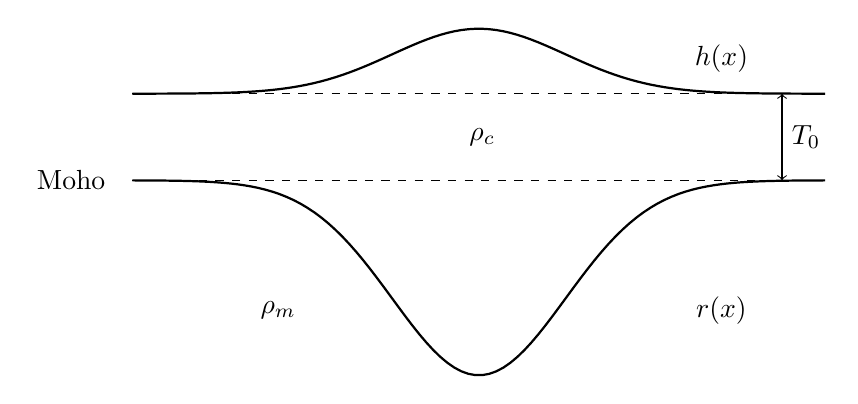
\begin{tikzpicture}[scale=1.1]

    % Parameters
    \def\A{0.75}      % topography amplitude
    \def\Tzero{1.0}  % reference crustal thickness
    \def\k{0.5}      % Gaussian width

    % Topography (Gaussian)
    \draw[thick, domain=-4:4, samples=100]
        plot (\x, {\A*exp(-\k*\x*\x)});

    % Reference surface (sea level)
    \draw[dashed] (-4,0) -- (4,0);

    % Moho (reference crustal thickness)
    \draw[dashed] (-4,-\Tzero) -- (4,-\Tzero);

    % Root (3x amplitude below Moho)
    \draw[thick, domain=-4:4, samples=100]
        plot (\x, {-\Tzero - 3*\A*exp(-\k*\x*\x)});

    % Label topography
    \node at (2.8,0.4) {$h(x)$};

    % Label root
    \node at (2.8,-2.5) {$r(x)$};

    % Label T0 with bracket
    \draw[<->] (3.5,0) -- (3.5,-\Tzero);

    \node[left] at (0.3,-0.5) {$\rho_c$};
    \node[left] at (-2,-2.5) {$\rho_m$};

    \node[right] at (3.5,-0.5*\Tzero) {$T_0$};

    % Label Moho
    \node[left] at (-4.2,-\Tzero) {Moho};

    \end{tikzpicture}
    \caption{A mountain with a topographic expression $h(x)$ and compensating root $r(x)$.}
\end{figure}

\section*{Tasks}

\begin{questions}
    \question{Part 1: Root Thickness}
    \begin{enumerate}[label=\roman*]
        \item Using the general mass-balance principle from Activity 5.A, write the pressure balance between the reference column ($T_0$, $\rho_c$, mantle below) and the topographic column ($T_0+h+r$, $\rho_c$), evaluated at the depth of compensation. Show that this reduces to
        \[
            \rho_c h = (\rho_m - \rho_c)\, r .
        \]
        \answerbox[6cm]

        \item Solve for the root thickness $r(x)$ in terms of $h(x)$.
        \answerbox[3cm]

        \item Is this compensation pattern consistent with one of the end-member models, Airy or Pratt, and if so why?
        \answerbox[3cm]
    \end{enumerate}

    \question{Part 2: Gravity of an Infinite Slab}
    Recall the infinite slab formula from Week~4: the gravitational attraction of an infinite horizontal slab of thickness $t$ and density $\rho$ is
    \[
        g = 2\pi G \rho t .
    \]
    \begin{enumerate}[label=\roman*]
        \item Write an expression for the gravitational effect of the topography.
        \answerbox[3cm]

        \item Write an expression for the gravitational effect of the crustal root. Carefully define the density contrast.
        \answerbox[3cm]
    \end{enumerate}

    \question{Part 3: Substitution and Simplification}
    \begin{enumerate}[label=\roman*]
        \item Substitute your expression for $r(x)$ into the root gravity term.
        \answerbox[5cm]

        \item Show that the total gravity effect of the topography plus its compensating root simplifies to:
        \[
            g_{\text{total}} = 0
        \]
        \answerbox[5cm]
    \end{enumerate}

    \question{Part 4: Practical Isostatic Correction}
    In practice, crustal thickness is not known everywhere. Instead, we assume a reference thickness $T_0$ and compute $r(x)$ from observed topography.
    \begin{enumerate}[label=\roman*]
        \item Explain why the isostatic correction is model-dependent.
        \answerbox[3cm]

        \item Write the final expression for the isostatic correction in terms of $h(x)$ only.

        You should show that the gravity effect of the compensating root is:
        \[
            g_{\text{root}} = -2\pi G \rho_c h
        \]
        and that, under perfect compensation, the combined effect of topography and root cancels exactly.
        \answerbox[3cm]
    \end{enumerate}

    \question{Extension (Optional)}
    \begin{enumerate}
        \item If a load is only partially compensated, does the topography--root cancellation from Part~3 still hold exactly? What would you expect to see in the residual gravity anomaly, and what does its sign tell you?
        \answerbox[3cm]

        \item Partial compensation of this kind arises physically from lithospheric flexure. Why does a rigid lithosphere leave short-wavelength loads less compensated than long-wavelength ones?
        \answerbox[3cm]
    \end{enumerate}
\end{questions}

\section*{Key Ideas}

\textbf{Under perfect compensation, topography and its root cancel exactly.} The gravity signal from a mountain ($+2\pi G\rho_c h$) is exactly cancelled by its deeper crustal root ($-2\pi G\rho_c h$). A perfectly compensated terrain therefore has no isostatic gravity anomaly --- any residual signal indicates incomplete compensation or lateral density variations.

\textbf{This crustal-thickness-only pattern is an end-member.} Constant crustal density with a compensating root is exactly the pattern you classified in Part 1 --- the same general balance would look different for a case with different fundamental assumptions.

\textbf{The isostatic correction depends on a model, not just data.} To apply the correction in practice we must assume a crustal density and a reference thickness $T_0$; both are uncertain. Different choices of these parameters produce different corrections, so the corrected gravity inherits model uncertainty.

\textbf{Flexural rigidity distributes the compensation laterally.} A rigid lithosphere can support loads over a finite wavelength range without immediate local isostatic adjustment. Short-wavelength topography is not compensated; long-wavelength topography is. The effective elastic thickness of the lithosphere controls where this transition occurs.

\end{activity}